\chapter{Células-Tronco, Regeneração e Envelhecimento}\label{ch:b3:stem-cells}

Corte a perna de um axolote e em dois meses ele terá feito crescer uma
nova, com osso, músculo, nervo e pele nos lugares certos, e voltará a
fazê-lo tantas vezes quantas você cortar. Corte uma planária em vinte
pedaços e cada um vira um verme inteiro em quinze dias, com o pedaço que
era cauda fazendo crescer uma cabeça com olhos e cérebro. Corte um dedo
humano acima da última articulação e ele fecha em cicatriz. E, no
entanto, o corpo humano não é sem renovação: a cada segundo ele faz dois
milhões de hemácias, o revestimento do intestino é substituído a cada
cinco dias, a pele a cada mês, e tudo isso descende de pequenas
populações de células que se dividem a vida toda sem se esgotar. Este
capítulo trata dessas células --- o que faz uma \omterm{def:b3:stem-cells:stem}{célula-tronco}, como seu
\omterm{def:b3:stem-cells:stem}{nicho} a mantém, como toda a hierarquia do sangue ou do intestino é
construída a partir dela ---, dos animais que conseguem refazer o que
nós não conseguimos e por quê, da descoberta de que qualquer célula pode
ser empurrada de volta ao estado embrionário por quatro genes, e do que
a aritmética da divisão celular tem a dizer sobre por que envelhecemos.

\section{O que é uma célula-tronco}

\begin{definition}[Células-tronco e sua hierarquia]\label{def:b3:stem-cells:stem}
\index{célula-tronco}\index{autorrenovação}\index{divisão assimétrica}\index{progenitor}\index{célula amplificadora de trânsito}\index{nicho}
Uma \emph{célula-tronco} tem duas propriedades definidoras: ela pode se
\emph{autorrenovar}, produzindo filhas que são células-tronco, e pode
produzir filhas que se diferenciam. Pode fazer as duas coisas de uma vez,
por \emph{divisão assimétrica}, uma filha de cada tipo, com o destino
decidido pela herança desigual de determinantes ou por qual filha
permanece em contato com o \emph{nicho} --- o microambiente de células
vizinhas, matriz e sinais que mantém uma célula como célula-tronco; ou
pode se dividir simetricamente, com algumas divisões dando duas
células-tronco e outras duas células em diferenciação, mantendo a
população constante em média. As filhas em diferenciação costumam passar
por estágios de \emph{progenitor} ou de \emph{amplificação de trânsito},
dividindo-se mais algumas vezes com potência cada vez mais estreita antes
de amadurecer: a hierarquia amplifica algumas poucas divisões lentas de
células-tronco numa produção grande e limita o número de divisões que
qualquer célula-tronco precisa fazer. As células-tronco adultas são raras
e lentas --- uma célula-tronco hematopoética se divide talvez uma vez por
ano, uma célula-tronco intestinal uma vez por dia --- e
\emph{multipotentes}, restritas às linhagens de seu tecido; as
células-tronco embrionárias, da massa celular interna do blastocisto, são
\emph{pluripotentes}, capazes de fazer todos os tecidos do corpo, mas não
a placenta.
\end{definition}

\begin{omfigure}
\begin{tikzpicture}[every node/.style={font=\scriptsize}, >=stealth]
  \node[draw, very thick, rounded corners, fill=omDef!25, align=center] (hsc) at (0,3.6) {célula-tronco hematopoética\\$\sim$\num{10000} num humano; divide-se $\sim$ uma vez por ano};
  \node[draw, thick, rounded corners, fill=omDef!12, align=center] (mpp) at (0,2.4) {progenitores multipotentes};
  \node[draw, thick, rounded corners, fill=omThm!15, align=center] (cmp) at (-3.2,1.2) {progenitor mieloide};
  \node[draw, thick, rounded corners, fill=omProp!20, align=center] (clp) at (3.2,1.2) {progenitor linfoide};
  \node[align=center, font=\tiny] (e) at (-5.4,-0.4) {eritrócitos\\$2\times 10^{11}$/dia};
  \node[align=center, font=\tiny] (pl) at (-3.6,-0.4) {plaquetas\\(megacariócitos)};
  \node[align=center, font=\tiny] (g) at (-1.8,-0.4) {granulócitos\\$10^{11}$/dia};
  \node[align=center, font=\tiny] (m) at (-0.2,-0.4) {monócitos,\\macrófagos};
  \node[align=center, font=\tiny] (b) at (1.8,-0.4) {células B};
  \node[align=center, font=\tiny] (t) at (3.4,-0.4) {células T};
  \node[align=center, font=\tiny] (nk) at (5.0,-0.4) {células NK};
  \draw[->, thick] (hsc) -- (mpp); \draw[->, thick] (mpp) -- (cmp); \draw[->, thick] (mpp) -- (clp);
  \foreach \x in {e,pl,g,m} { \draw[->, thick] (cmp) -- (\x); }
  \foreach \x in {b,t,nk} { \draw[->, thick] (clp) -- (\x); }
  \draw[->, thick, omDef!70!black] (hsc.west) .. controls (-3.0,4.4) and (-3.0,3.0) .. (hsc.south west) node[pos=0.5, left, font=\tiny, omDef!70!black, align=right] {autorrenovação};
  \node[right, align=left, font=\tiny] at (4.4,3.6) {cada nível se divide mais vezes\\e tem potência mais estreita;\\$\sim 20$ divisões da célula-tronco\\à hemácia, de modo que uma divisão\\da célula-tronco rende $\sim 10^{6}$ células};
\end{tikzpicture}

{\small A hierarquia hematopoética. Alguns milhares de células-tronco
lentas na medula alimentam \omterm{def:b3:stem-cells:stem}{progenitores} que se dividem depressa e se
comprometem progressivamente, de modo que a produção de um trilhão de
células por dia quase nada custa às células-tronco.}
\end{omfigure}

\begin{proof}[Evidência]
Till e McCulloch (1961) injetaram células de medula em camundongos
irradiados de modo letal e contaram os nódulos que apareciam no baço dez
dias depois: cada um era uma colônia de células sanguíneas de várias
linhagens, com número proporcional às células injetadas, e marcar os
cromossomos das células doadoras mostrou que cada colônia era um clone
--- uma única célula tinha feito hemácias, granulócitos e plaquetas, e
algumas colônias continham células capazes de semear novas colônias num
segundo camundongo: \omterm{def:b3:stem-cells:stem}{autorrenovação} e multipotência numa só célula, a
definição operacional de uma \omterm{def:b3:stem-cells:stem}{célula-tronco} e a base do transplante de
medula óssea. Barker e Clevers (2007) marcaram com uma cor hereditária as
células que expressam o gene \emph{Lgr5} na base das criptas intestinais
e observaram, ao longo de semanas, a cor subir a cripta e preencher
vilosidades inteiras: as células marcadas eram as células-tronco do
intestino e uma delas, cultivada num gel com os três fatores de
crescimento certos, cresceu num intestino em miniatura, um
\emph{\omterm{def:b3:stem-cells:pluripotency}{organoide}}, com criptas e vilosidades próprias (Sato, 2009).
\end{proof}

\begin{proposition}[O nicho e a cripta]\label{prop:b3:stem-cells:crypt}
\index{cripta}\index{Lgr5}\index{célula de Paneth}\index{sinalização Wnt}\index{deriva neutra}
A \emph{cripta} intestinal é o \omterm{def:b3:stem-cells:stem}{nicho} mais bem compreendido. Em sua base,
cerca de catorze células-tronco \emph{Lgr5} ficam encaixadas entre
\omterm{prop:b3:stem-cells:crypt}{células de Paneth}, que secretam os sinais Wnt e Notch e os fatores de
crescimento que as mantêm células-tronco; uma \omterm{def:b3:stem-cells:stem}{célula-tronco} empurrada
para cima, fora de contato com as \omterm{prop:b3:stem-cells:crypt}{células de Paneth}, perde o sinal em
poucos diâmetros celulares e se torna uma \omterm{def:b3:stem-cells:stem}{célula amplificadora de
trânsito}, que se divide quatro ou cinco vezes na cripta e então se
diferencia nas células absortivas e secretoras que migram pela vilosidade
acima e são descamadas de sua ponta cinco dias depois. As células-tronco
se dividem simetricamente, cerca de uma vez por dia, e competem pelo
espaço limitado do \omterm{def:b3:stem-cells:stem}{nicho}: por acaso um clone se expande e os outros são
perdidos, de modo que, em poucos meses, toda cripta descende de uma única
\omterm{def:b3:stem-cells:stem}{célula-tronco} --- \emph{\omterm{prop:b3:stem-cells:crypt}{deriva neutra}} na escala de uma cripta, um
passeio aleatório com fronteiras absorventes. O \omterm{def:b3:stem-cells:stem}{nicho}, e não a célula,
guarda o caráter de tronco: ponha uma célula diferenciada de volta em
contato com os sinais de Paneth depois de uma lesão e ela pode reverter;
tire a \omterm{def:b3:stem-cells:stem}{célula-tronco} de lá e lhe dê os sinais numa placa e ela faz um
\omterm{def:b3:stem-cells:pluripotency}{organoide}. A medula óssea, os folículos pilosos, o testículo e as zonas
de células-tronco neurais do encéfalo seguem a mesma lógica com sinais
diferentes.
\end{proposition}
\begin{proof}[Evidência]
Snippert e colaboradores (2010) marcaram células-tronco de cripta com um
``confete'' de quatro cores aleatórias; as criptas eram multicoloridas a
princípio e já eram de cor única em alguns meses, a uma taxa compatível
com divisão simétrica e competição neutra entre cerca de catorze células
--- e não com \omterm{def:b3:stem-cells:stem}{divisão assimétrica}, que teria mantido toda cor
indefinidamente. Remover as \omterm{prop:b3:stem-cells:crypt}{células de Paneth} encolhe o conjunto de
células-tronco; remover o sinal Wnt esvazia a cripta em dias.
\end{proof}

\begin{omfigure}
\begin{tikzpicture}[every node/.style={font=\scriptsize}, >=stealth]
  % crypt-villus
  \draw[very thick, omDef] (0,-2.6) .. controls (0,-0.4) and (0.4,0) .. (0.8,0) -- (0.8,3.6) .. controls (0.8,4.1) and (1.6,4.1) .. (1.6,3.6) -- (1.6,0) .. controls (2.0,0) and (2.4,-0.4) .. (2.4,-2.6);
  \draw[very thick, omDef] (0,-2.6) arc[start angle=180, end angle=360, radius=1.2];
  % stem cells at base
  \foreach \a in {200,230,260,290,320} { \fill[omThm!60] ({1.2+1.05*cos(\a)},{-2.6+1.05*sin(\a)}) circle (0.14); }
  \foreach \a in {215,245,275,305} { \fill[omMeth!60] ({1.2+0.75*cos(\a)},{-2.6+0.75*sin(\a)}) circle (0.13); }
  \node[right, align=left, font=\tiny] at (2.6,-3.4) {base: $\sim 14$ células-tronco \emph{Lgr5} (vermelho)\\encaixadas entre células de Paneth (verde),\\que fornecem Wnt, Notch, EGF};
  % TA zone
  \foreach \y in {-1.8,-1.3,-0.8,-0.3} { \fill[omProp!50] (0.35,\y) circle (0.11); \fill[omProp!50] (2.05,\y) circle (0.11); }
  \node[right, align=left, font=\tiny] at (2.6,-1.1) {zona de amplificação de trânsito:\\4--5 divisões, uma por dia,\\além dos sinais de Paneth};
  % villus cells
  \foreach \y in {0.4,1.0,1.6,2.2,2.8} { \fill[omDef!40] (0.95,\y) circle (0.1); \fill[omDef!40] (1.45,\y) circle (0.1); }
  \node[right, align=left, font=\tiny] at (2.6,1.8) {vilosidade: células diferenciadas\\migram para cima e são descamadas\\da ponta após $\sim 5$ dias};
  \node[left, font=\tiny] at (-0.1,-2.6) {cripta}; \node[left, font=\tiny] at (0.7,3.9) {ponta da vilosidade};
  % confetti panel
  \begin{scope}[shift={(8.8,0.2)}]
    \node[above, align=center] at (0,1.3) {deriva neutra no nicho};
    \foreach \i/\cols in {0/{omDef!60,omThm!60,omMeth!60,omProp!60,omDef!60,omThm!60}, 1/{omDef!60,omDef!60,omThm!60,omThm!60,omThm!60,omProp!60}, 2/{omThm!60,omThm!60,omThm!60,omThm!60,omDef!60,omThm!60}, 3/{omThm!60,omThm!60,omThm!60,omThm!60,omThm!60,omThm!60}} {
      \foreach [count=\j] \c in \cols { \fill[\c] ({\j*0.36-1.26},{1.0-\i*0.7}) circle (0.15); }
    }
    \node[left, font=\tiny] at (-1.35,1.0) {semana 0}; \node[left, font=\tiny] at (-1.35,0.3) {semana 4}; \node[left, font=\tiny] at (-1.35,-0.4) {semana 12}; \node[left, font=\tiny] at (-1.35,-1.1) {meses};
    \node[below, align=center, font=\tiny] at (0,-1.75) {os clones competem por um número fixo\\de lugares; um vence por acaso};
  \end{scope}
\end{tikzpicture}

{\small A cripta como \omterm{def:b3:stem-cells:stem}{nicho}. Ser tronco é um lugar: as células em contato
com os sinais das \omterm{prop:b3:stem-cells:crypt}{células de Paneth} continuam células-tronco; as
empurradas para fora do contato começam a viagem de cinco dias até a
ponta da vilosidade. Marcadas com cores aleatórias, as células-tronco de
uma cripta derivam para um único clone em poucos meses.}
\end{omfigure}

\section{Pluripotência e reprogramação}

\begin{definition}[Embrionárias, induzidas e cultivadas]\label{def:b3:stem-cells:pluripotency}
\index{célula-tronco embrionária}\index{pluripotência}\index{célula-tronco pluripotente induzida}\index{reprogramação}\index{organoide}
As \emph{células-tronco embrionárias} (Evans, Kaufman, Martin, 1981, em
camundongo; Thomson, 1998, em humanos) são células da massa celular
interna mantidas em divisão em cultura sem se diferenciar, por sinais
(LIF, ou FGF e activina) que mantêm um núcleo de fatores de transcrição
--- Oct4, Sox2, Nanog --- que se ativam mutuamente e reprimem os genes de
toda linhagem. Injetadas num blastocisto, elas se juntam ao embrião e
contribuem para todos os seus tecidos, inclusive a linhagem germinativa,
que é como se faz o camundongo \omterm{def:b3:genetic-engineering:transgenic}{nocaute}: altere um gene nas células e faça
um camundongo a partir delas. A transferência nuclear do volume do Ano~2
mostrou que um núcleo diferenciado pode ser reiniciado pelo citoplasma do
ovo; Takahashi e Yamanaka (2006) descobriram o que faz esse reinício. De
vinte e quatro genes candidatos, quatro --- \emph{Oct4}, \emph{Sox2},
\emph{Klf4}, \emph{c-Myc} ---, introduzidos juntos por \omterm{def:b3:virology:virus}{vírus} em
fibroblastos de pele, converteram cerca de uma célula em mil, ao longo de
três semanas, numa \emph{\omterm{def:b3:stem-cells:stem}{célula-tronco} pluripotente induzida}
indistinguível de uma embrionária, capaz de formar todos os tecidos e um
camundongo inteiro. A \emph{reprogramação} é lenta e ineficiente porque
os fatores precisam abrir a \omterm{def:b3:chromatin-epigenetics:nucleosome}{cromatina} fechada por anos de diferenciação,
e as células passam por uma fase estocástica em que a maioria empaca; ela
é também, em princípio, uma rota das próprias células de um paciente até
qualquer tecido. Acrescente os sinais certos na ordem certa e células
pluripotentes numa placa recapitulam o desenvolvimento: músculo cardíaco
que bate, neurônios dopaminérgicos para transplante num encéfalo
parkinsoniano, células retinianas, e \emph{organoides} --- tecidos
tridimensionais auto-organizados de alguns milímetros, de intestino, rim,
fígado e cérebro, com a arquitetura e os tipos celulares do órgão, nos
quais o desenvolvimento e as doenças humanas podem ser observados e
fármacos testados.
\end{definition}

\begin{omfigure}
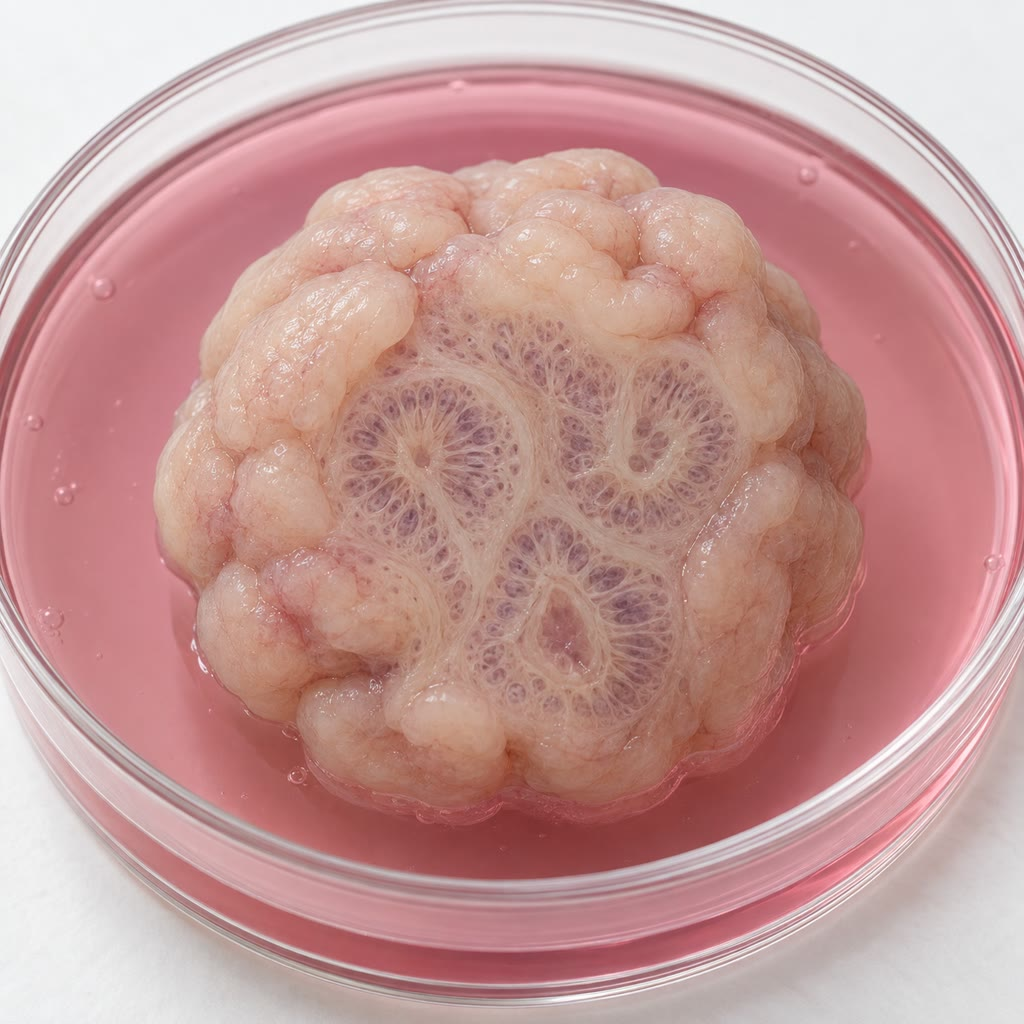
\includegraphics[width=0.4\linewidth]{images/book5/ai/b5-24-brain-organoid.jpg}\hspace{0.04\linewidth}
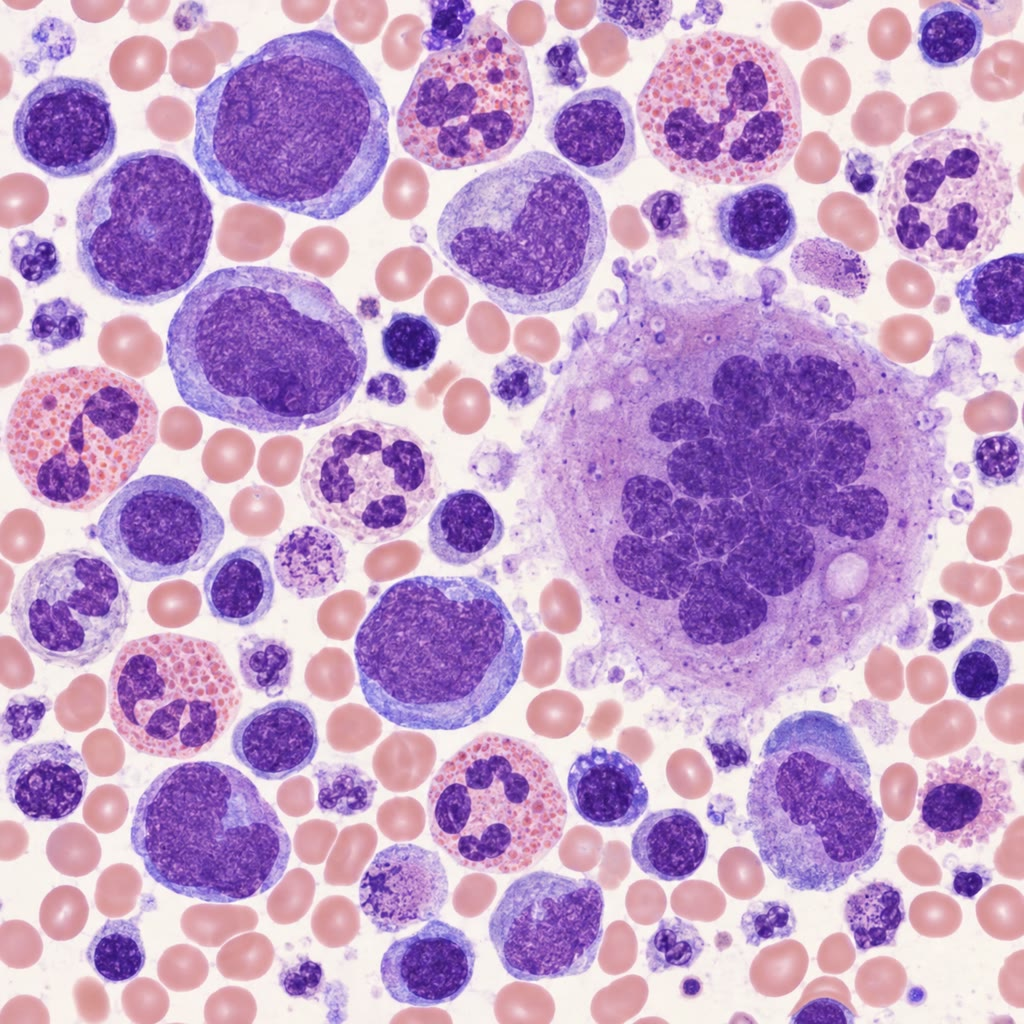
\includegraphics[width=0.4\linewidth]{images/book5/ai/b5-24-bone-marrow-smear.jpg}

{\small À esquerda: um \omterm{def:b3:stem-cells:pluripotency}{organoide} cerebral cultivado a partir de células
pluripotentes humanas --- alguns milímetros de tecido auto-organizado
semelhante ao córtex, com cavidades semelhantes a ventrículos e neurônios
em camadas. À direita: um esfregaço de medula óssea, a hierarquia da
primeira figura vista de uma só vez: blastos, granulócitos em maturação,
precursores de hemácias e um megacariócito.}
\end{omfigure}

\begin{method}[Rastreamento de linhagem]\label{met:b3:stem-cells:tracing}
\index{rastreamento de linhagem}\index{recombinase Cre}
Para descobrir quais células são as células-tronco de um tecido: (1)
escolha um gene expresso pelas células candidatas e ponha sob seu
promotor uma recombinase indutível (Cre-ER, ativa apenas quando se dá
tamoxifeno); (2) no mesmo animal, um gene repórter que fica
permanentemente ativo quando a recombinase corta dele um cassete de
parada --- uma cor herdada por todos os descendentes; (3) dê uma dose
única de tamoxifeno para marcar as células candidatas num momento; (4)
colha tecido em intervalos e avalie os clones marcados: um clone que
cresce, persiste por meses e contém todos os tipos celulares do tecido
veio de uma \omterm{def:b3:stem-cells:stem}{célula-tronco}; um clone descamado em uma semana veio de uma
célula de trânsito. (5) Com um repórter multicolorido, acompanhe a
competição entre clones. (6) Teste a função diretamente matando as
células marcadas com um receptor de toxina expresso sob o mesmo promotor,
e veja se o tecido deixa de se renovar.
\end{method}

\section{Regeneração}

\begin{definition}[Como os animais refazem]\label{def:b3:stem-cells:regeneration}
\index{regeneração}\index{neoblasto}\index{blastema}\index{desdiferenciação}\index{crescimento compensatório}
A regeneração toma três rotas. A \emph{Hydra} e a planária dependem de
células-tronco pluripotentes adultas: os \emph{neoblastos} de uma
planária, um quinto de suas células, são as únicas células em divisão que
ela tem, migram para uma ferida e reconstroem qualquer parte faltante,
guiados por sinais posicionais (um gradiente de Wnt diz ao pedaço que
extremidade é a cauda; bloqueie-o e um pedaço de cauda faz crescer uma
segunda cabeça). As salamandras reconstroem um membro a partir de um
\emph{blastema}, uma tampa de células em divisão no coto, formada em boa
parte por \emph{desdiferenciação}: as fibras musculares se fragmentam em
células mononucleadas, as células cartilaginosas e conjuntivas voltam a
um estado de \omterm{def:b3:stem-cells:stem}{progenitor}, cada uma lembrando seu tecido de origem e sua
posição ao longo do membro, e o blastema roda de novo o programa
embrionário do membro sob a epiderme da ferida e os nervos, cuja presença
é exigida (desnerve o coto e nada cresce). Os peixes-zebra refazem
nadadeiras e coração do mesmo modo, com as células musculares cardíacas
sobreviventes se dividindo para repor um quinto do ventrículo em um mês.
Os mamíferos fazem pouco disso: o fígado refaz sua massa depois de
removidos dois terços, mas pela divisão das células remanescentes no
lugar (\emph{crescimento compensatório}), e não reconstruindo os lobos
perdidos; uma ponta de dedo se regenera em crianças; os chifres do veado
crescem de novo a cada ano a partir de um periósteo de células-tronco.
Por que não mais que isso é uma questão de compromissos: a resposta
mamífera à ferida --- coagulação rápida, \omterm{def:b3:innate-immunity:inflammation}{inflamação}, cicatriz fibroblástica
--- fecha depressa uma ferida contra a infecção e a perda de sangue, e a
cicatriz inviabiliza o blastema; e células capazes de se desdiferenciar e
se dividir à vontade são células capazes de virar \omterm{def:b3:cancer-biology:hallmarks}{cânceres}, um risco que
um animal longevo e de sangue quente pode não bancar.
\end{definition}

\begin{omfigure}
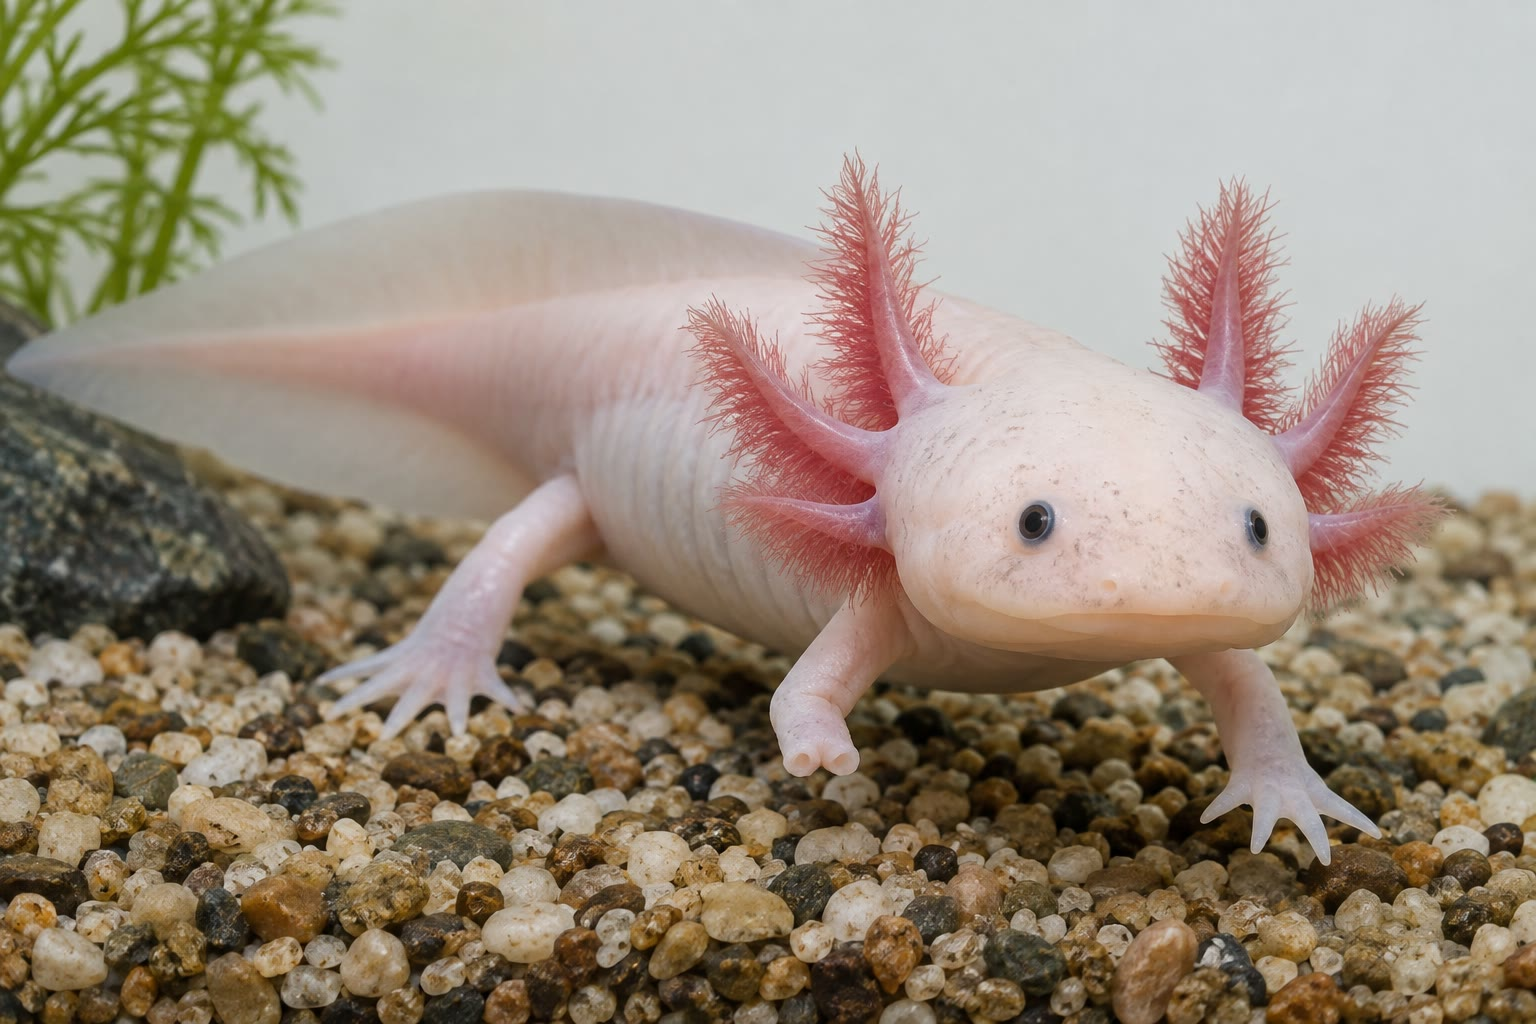
\includegraphics[width=0.46\linewidth]{images/book5/ai/b5-24-axolotl.jpg}\hspace{0.04\linewidth}
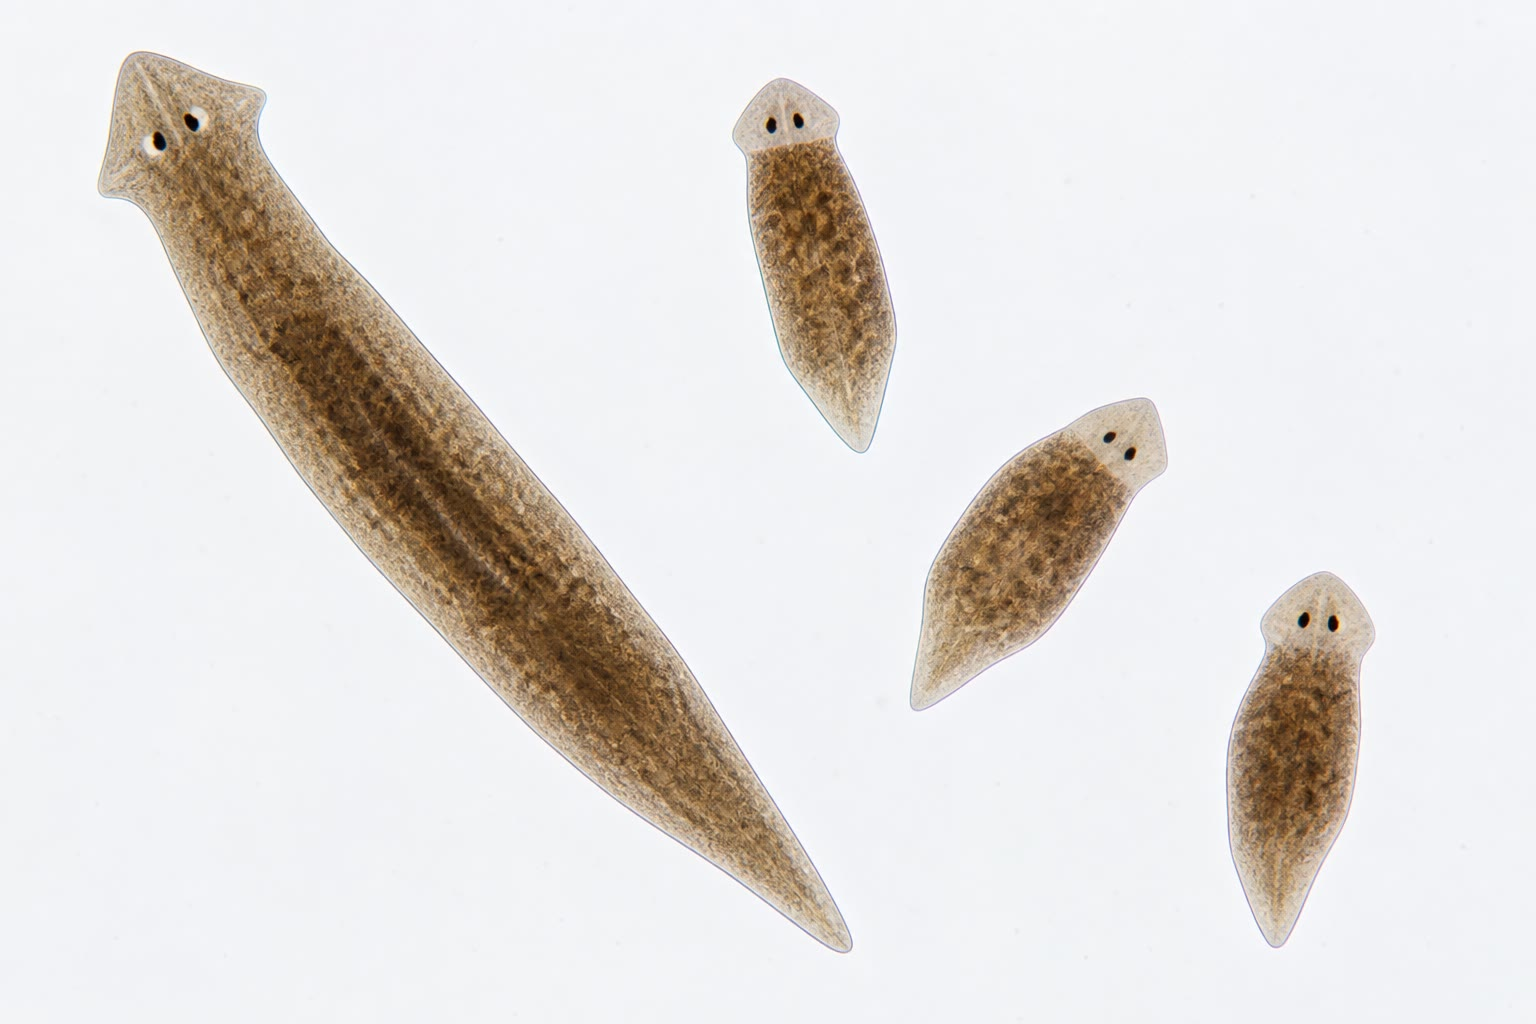
\includegraphics[width=0.46\linewidth]{images/book5/ai/b5-24-planarian-regeneration.jpg}

{\small À esquerda: um axolote, que refaz um membro em dois meses a
partir de um \omterm{def:b3:stem-cells:regeneration}{blastema} de células desdiferenciadas e pode fazê-lo a vida
toda. À direita: uma planária cortada em pedaços, cada pedaço refazendo
um verme completo a partir de seus \omterm{def:b3:stem-cells:regeneration}{neoblastos} em duas semanas.}
\end{omfigure}

\begin{proof}[Evidência]
Morgan (1898) cortou planárias em 279 pedaços e descobriu que cada um
refazia um verme inteiro, até um limite de cerca de um centésimo do
corpo; Reddien e colaboradores (2011) transplantaram um único \omterm{def:b3:stem-cells:regeneration}{neoblasto}
para um verme irradiado de modo letal e o restauraram por inteiro --- uma
célula, todos os tecidos. Kragl e colaboradores (2009) fizeram axolotes
com um tecido marcado em verde de cada vez e os enxertaram em hospedeiros
não marcados: após a amputação, o músculo verde deu origem apenas a
músculo, e a cartilagem verde apenas a cartilagem --- o \omterm{def:b3:stem-cells:regeneration}{blastema} não é um
reservatório de células pluripotentes, mas um conjunto de \omterm{def:b3:stem-cells:stem}{progenitores}
restritos a linhagens, cada um desdiferenciado apenas até o \omterm{def:b3:stem-cells:stem}{progenitor} de
seu próprio tecido. Singer (1952) mostrou que um membro de salamandra só
se regenera se um número limiar de fibras nervosas alcança o coto, e que
desviar um nervo para uma ferida no flanco fazia um membro crescer ali.
\end{proof}

\section{A aritmética do envelhecimento}

\begin{theorem}[Telômeros e o limite de Hayflick]\label{thm:b3:stem-cells:hayflick}
\index{telômero}\index{limite de Hayflick}\index{problema da replicação das extremidades}\index{telomerase}\index{senescência replicativa}
Cada cromossomo termina num \emph{telômero}, vários quilobases da
repetição TTAGGG. Como a DNA polimerase não consegue completar o último
trecho da fita retardada (o \emph{problema da replicação das
extremidades}), cada divisão encurta cada telômero em $\Delta \approx$
\qtyrange{50}{100}{bp}. Partindo de $L_{0} \approx \qty{10}{kb}$ e
disparando a \emph{\omterm{thm:b3:stem-cells:hayflick}{senescência replicativa}} --- uma parada permanente
imposta pela p53 --- quando o telômero mais curto chega a
$L_{\text{crit}} \approx \qty{4}{kb}$, uma linhagem celular pode se
dividir no máximo
\[
n_{\max} = \frac{L_{0} - L_{\text{crit}}}{\Delta} \approx \frac{6000}{50\text{--}100} \approx 60\text{--}120
\]
vezes: o \emph{\omterm{thm:b3:stem-cells:hayflick}{limite de Hayflick}}, as cinquenta e tantas duplicações
populacionais que os fibroblastos humanos completam em cultura antes de
parar. A enzima \emph{\omterm{def:b3:cancer-biology:telomerase}{telomerase}}, uma transcriptase reversa com molde de
RNA, reestende as extremidades; ela é ativa na linhagem germinativa, em
células-tronco embrionárias e em muitas adultas, e em \qty{90}{\%} dos
\omterm{def:b3:cancer-biology:hallmarks}{cânceres}, que escaparam do limite ao religá-la. Uma \omterm{def:b3:stem-cells:stem}{célula-tronco} que se
divide $d$ vezes por ano com a \omterm{def:b3:cancer-biology:telomerase}{telomerase} compensando uma fração $f$ da
perda tem $n_{\max} = (L_{0} - L_{\text{crit}})/[(1 - f)\Delta]$
divisões, e uma vida de $n_{\max}/d$ anos: com $f = 0.7$, $\Delta
= 60$,
$d = 1$, uns 330 anos para uma \omterm{def:b3:stem-cells:stem}{célula-tronco} hematopoética --- mas seus
\omterm{def:b3:stem-cells:stem}{progenitores}, com a \omterm{def:b3:cancer-biology:telomerase}{telomerase} desligada e vinte divisões até uma
hemácia, gastam um quinto de sua reserva a cada linhagem, e é por isso
que as células sanguíneas dos idosos têm telômeros mais curtos que as dos
jovens, em cerca de \qty{30}{bp} por ano.
\end{theorem}
\begin{proof}
A perda por divisão é um comprimento fixo, de modo que o comprimento do
telômero cai linearmente com o número de divisões, $L_{n} = L_{0} - n\Delta$, e chega a $L_{\text{crit}}$ em $n = (L_{0} - L_{\text{crit}})/\Delta$; com compensação parcial a perda líquida por
divisão é $(1 - f)\Delta$. Hayflick e Moorhead (1961) mostraram que
fibroblastos humanos normais param depois de cerca de cinquenta
duplicações, quaisquer que sejam as condições de cultura, que células
congeladas após vinte duplicações e descongeladas completam apenas as
trinta restantes --- elas contam divisões, e não tempo --- e que o limite
é menor para células de doadores idosos. Harley, Futcher e Greider (1990)
mediram os telômeros encurtando com as duplicações em cultura e com a
idade do doador; Bodnar e colaboradores (1998) puseram \omterm{def:b3:cancer-biology:telomerase}{telomerase} em
células normais e elas se dividiram além do limite indefinidamente sem se
tornar cancerosas, o que estabeleceu o telômero como o relógio.
\end{proof}

\begin{omfigure}
\begin{tikzpicture}
\begin{axis}[
  width=0.62\linewidth, height=5.4cm,
  axis x line=bottom, axis y line=left,
  xmin=0, xmax=120, ymin=0, ymax=11,
  xlabel={duplicações populacionais}, ylabel={comprimento do telômero (kb)},
  xlabel style={font=\small, at={(axis description cs:0.5,-0.12)}, anchor=north}, ylabel style={font=\small},
  tick label style={font=\small}, xtick={0,30,60,90,120}, ytick={4,7,10},
  clip=false,
]
\addplot[very thick, omDef, domain=0:60, samples=2] {10-0.1*x};
\addplot[very thick, omThm, domain=0:120, samples=2] {10-0.05*x};
\addplot[very thick, omMeth!70!black, domain=0:120, samples=2] {10-0.015*x};
\draw[dashed, gray] (axis cs:0,4) -- (axis cs:120,4); \node[font=\scriptsize, gray, anchor=north west] at (axis cs:2,3.9) {senescência em $L_{\text{crit}} = \qty{4}{kb}$};
\node[font=\scriptsize, omDef, anchor=south west] at (axis cs:63,4.3) {$\Delta = \qty{100}{bp}$: 60 duplicações};
\node[font=\scriptsize, omThm, anchor=west] at (axis cs:70,8.0) {$\Delta = \qty{50}{bp}$: 120};
\node[font=\scriptsize, omMeth!70!black, anchor=south west, align=left] at (axis cs:78,9.3) {telomerase compensando\\\qty{70}{\%}: 400};
\fill[omDef] (axis cs:60,4) circle (2pt); \fill[omThm] (axis cs:120,4) circle (2pt);
\end{axis}
\end{tikzpicture}

{\small Os telômeros como contador de divisões. Uma perda fixa por
divisão dá uma reta; onde ela cruza o comprimento crítico a linhagem
para. A \omterm{def:b3:cancer-biology:telomerase}{telomerase} achata a inclinação e, plenamente ativa, abole o
limite --- na linhagem germinativa e nos \omterm{def:b3:cancer-biology:hallmarks}{cânceres}.}
\end{omfigure}

\begin{proposition}[A lei de Gompertz]\label{prop:b3:stem-cells:gompertz}
\index{lei de Gompertz}\index{taxa de mortalidade}\index{marcas do envelhecimento}\index{célula senescente}
Acima de cerca de trinta anos a \omterm{prop:b3:stem-cells:gompertz}{taxa de mortalidade} humana $\mu(t)$ --- a
probabilidade de morrer no ano seguinte --- dobra a cada oito anos:
$\mu(t) =
\mu_{0}\,\mathrm{e}^{\gamma(t - t_{0})}$ com $\gamma = \ln 2/8 \approx
\qty{0.087}{yr^{-1}}$ (Gompertz, 1825). A sobrevivência até a
idade $t$ é então
\[
S(t) = \exp\!\Bigl[-\frac{\mu_{0}}{\gamma}\bigl(\mathrm{e}^{\gamma(t - t_{0})} - 1\bigr)\Bigr],
\]
uma curva plana por décadas e depois em queda íngreme, com uma
expectativa mediana de vida $t_{1/2} = t_{0} + \gamma^{-1}\ln(1 + \gamma\ln 2/\mu_{0})$: para $\mu_{0} = 10^{-3}$ por ano aos trinta,
cerca de $30 + 47 = 77$ anos. A mesma lei, com constantes diferentes,
vale para camundongos (tempo de duplicação de três meses), cães, moscas e
vermes: envelhecer é uma elevação exponencial da vulnerabilidade, e não
um relógio que para. A biologia por trás do expoente é um conjunto de
\emph{marcas} que interagem: dano acumulado ao DNA e deriva \omterm{def:b3:chromatin-epigenetics:epigenetics}{epigenética},
desgaste dos telômeros, perda da proteostase, declínio mitocondrial,
esgotamento dos reservatórios de células-tronco, o acúmulo de
\emph{\omterm{prop:b3:stem-cells:gompertz}{células senescentes}} que já não se dividem mas secretam sinais
inflamatórios, e a \omterm{def:b3:innate-immunity:inflammation}{inflamação} crônica; em camundongos, eliminar \omterm{prop:b3:stem-cells:gompertz}{células
senescentes} ou restringir calorias prolonga a vida, e em vermes uma única
mutação na via semelhante à da \omterm{def:b3:endocrinology:glucose}{insulina} a dobra. Se o expoente pode ser
reduzido em humanos, em vez da constante $\mu_{0}$, que a medicina já
reduziu dez vezes em um século, é a questão em aberto.
\end{proposition}
\begin{proof}
Se $\mu$ é o risco instantâneo, $\mathrm{d}S/\mathrm{d}t = -\mu(t)S$, de
modo que $\ln S =
-\int_{t_{0}}^{t}\mu = -(\mu_{0}/\gamma)(\mathrm{e}^{\gamma(t-t_{0})} -
1)$. Fazendo $S = 1/2$:
$\mathrm{e}^{\gamma(t-t_{0})} = 1 + \gamma\ln 2/
\mu_{0}$, donde a
mediana; com $\gamma = 0.087$ e $\mu_{0} =
10^{-3}$, $\ln(1 + 60) = 4.1$
e $t - t_{0} = 47$. A lei empírica é o ajuste de Gompertz às tábuas de
vida inglesas; que ela descreva tantas espécies com uma forma comum e
constantes específicas de cada uma é admitido aqui como o resumo de um
século de demografia.
\end{proof}

\begin{omfigure}
\begin{tikzpicture}
\begin{semilogyaxis}[
  width=0.5\linewidth, height=5.2cm,
  axis x line=bottom, axis y line=left,
  xmin=20, xmax=100, ymin=0.0003, ymax=1,
  xlabel={idade (anos)}, ylabel={taxa de mortalidade por ano},
  xlabel style={font=\small, at={(axis description cs:0.5,-0.12)}, anchor=north}, ylabel style={font=\small},
  tick label style={font=\small}, xtick={30,50,70,90}, ytick={0.001,0.01,0.1,1}, yticklabels={0.001,0.01,0.1,1},
  clip=false,
]
\addplot[very thick, omDef, domain=30:100, samples=2] {0.001*exp(0.0866*(x-30))};
\node[font=\scriptsize, omDef, anchor=north west, align=left] at (axis cs:32,0.3) {$\mu = \mu_{0}\,\mathrm{e}^{\gamma(t-30)}$\\dobrando a cada 8 anos};
\end{semilogyaxis}
\begin{axis}[
  at={(0.55\linewidth,0)}, anchor=south west,
  width=0.43\linewidth, height=5.2cm,
  axis x line=bottom, axis y line=left,
  xmin=20, xmax=110, ymin=0, ymax=1.05,
  xlabel={idade (anos)}, ylabel={fração sobrevivente},
  xlabel style={font=\small, at={(axis description cs:0.5,-0.12)}, anchor=north}, ylabel style={font=\small},
  tick label style={font=\small}, xtick={30,50,77,100}, ytick={0.5,1},
  clip=false,
]
\addplot[very thick, omThm, domain=30:110, samples=80] {exp(-(0.001/0.0866)*(exp(0.0866*(x-30))-1))};
\draw[dashed, gray] (axis cs:77,0) -- (axis cs:77,0.5) -- (axis cs:20,0.5);
\node[font=\scriptsize, omThm, anchor=north east, align=right] at (axis cs:75,0.45) {mediana\\77 anos};
\end{axis}
\end{tikzpicture}

{\small A \omterm{prop:b3:stem-cells:gompertz}{lei de Gompertz}. À esquerda: num eixo logarítmico a \omterm{prop:b3:stem-cells:gompertz}{taxa de
mortalidade} é uma reta dos trinta em diante. À direita: a curva de
sobrevivência que daí decorre --- um platô e depois um despenhadeiro, com
a mediana onde a integral do risco alcança $\ln 2$.}
\end{omfigure}

\begin{remark}[A renovação e seu preço]\label{rem:b3:stem-cells:remark}
Um corpo que se renova precisa manter células capazes de se dividir
indefinidamente, e células capazes de se dividir indefinidamente são a
matéria-prima do \omterm{def:b3:cancer-biology:hallmarks}{câncer}; um corpo que se protege do \omterm{def:b3:cancer-biology:hallmarks}{câncer} contando
divisões e impondo \omterm{def:b3:cell-cycle-apoptosis:other}{senescência} precisa, com o tempo, ficar sem células
capazes de se dividir. A hierarquia de células-tronco é uma solução ---
poucas células lentas protegidas em \omterm{def:b3:stem-cells:stem}{nichos}, muitas células rápidas que
logo morrem --- e o \omterm{thm:b3:stem-cells:hayflick}{limite de Hayflick} é outra, e a exponencial de
Gompertz é a soma de seus custos. A salamandra paga de outro jeito: ela
tolera células que se desdiferenciam e refaz uma perna, e é de sangue
frio, lenta e raramente vive o bastante para pagar a conta do \omterm{def:b3:cancer-biology:hallmarks}{câncer}. As
células com que você nasceu não são, em sua maior parte, as células que
você tem; as que fizeram as substitutas são as que você precisa manter.
\end{remark}

\section{Exercícios}

\begin{exercise}[$\star$]\label{exo:b3:stem-cells:1}
Defina \omterm{def:b3:stem-cells:stem}{autorrenovação}, potência, \omterm{def:b3:stem-cells:stem}{nicho} e \omterm{def:b3:stem-cells:stem}{célula amplificadora de
trânsito}, e dê um exemplo de cada um no intestino.
\end{exercise}

\begin{exercise}[$\star$]\label{exo:b3:stem-cells:2}
O que o ensaio de colônias esplênicas mostrou, e que propriedade de uma
\omterm{def:b3:stem-cells:stem}{célula-tronco} exigiu um segundo camundongo para ser demonstrada?
\end{exercise}

\begin{exercise}[$\star$]\label{exo:b3:stem-cells:3}
Nomeie os quatro fatores de Yamanaka e explique por que a \omterm{def:b3:stem-cells:pluripotency}{reprogramação}
leva semanas e dá certo num milésimo das células.
\end{exercise}

\begin{exercise}[$\star$]\label{exo:b3:stem-cells:4}
Contraste as rotas da planária e da salamandra para a \omterm{def:b3:stem-cells:regeneration}{regeneração}, e diga
o que os experimentos de enxertia de Kragl mostraram sobre o \omterm{def:b3:stem-cells:regeneration}{blastema}.
\end{exercise}

\begin{exercise}[$\star\star$]\label{exo:b3:stem-cells:5}
Os telômeros começam em \qty{11}{kb}, a \omterm{def:b3:cell-cycle-apoptosis:other}{senescência} ocorre em
\qty{5}{kb}, e a perda é de \qty{75}{bp} por divisão. \omterm{thm:b3:stem-cells:hayflick}{Limite de Hayflick}?
Células de um doador de 70 anos têm \qty{8}{kb}: duplicações restantes?
Se a \omterm{def:b3:cancer-biology:telomerase}{telomerase} compensar \qty{60}{\%} da perda, qual é o limite?
\end{exercise}

\begin{exercise}[$\star\star$]\label{exo:b3:stem-cells:6}
Uma cripta abriga 14 células-tronco que se dividem uma vez por dia,
alimentando células de trânsito que se dividem mais 4 vezes, e a cripta
fornece \num{300} células por dia à sua vilosidade. Confira a aritmética:
quantas divisões de células-tronco por dia produzem filhas em
diferenciação, e a quantas células-tronco isso equivale em divisões?
\end{exercise}

\begin{exercise}[$\star\star$]\label{exo:b3:stem-cells:7}
O corpo faz $2\times 10^{11}$ hemácias por dia, cada uma o produto de
cerca de 20 divisões a partir de uma \omterm{def:b3:stem-cells:stem}{célula-tronco}. Quantas divisões de
células-tronco por dia isso exige e, com \num{10000} células-tronco, com
que frequência cada uma se divide? Compare com o ``cerca de uma vez por
ano'' observado e explique a discrepância.
\end{exercise}

\begin{exercise}[$\star\star$]\label{exo:b3:stem-cells:8}
Com $\gamma = \qty{0.087}{yr^{-1}}$ e $\mu_{0} = 10^{-3}$ aos trinta,
calcule a \omterm{prop:b3:stem-cells:gompertz}{taxa de mortalidade} aos 50, 70 e 90, a sobrevivência até 70 e
90, e a expectativa mediana de vida. O que reduzir $\mu_{0}$ à metade faz
com a mediana? E o que faz reduzir $\gamma$ à metade?
\end{exercise}

\begin{exercise}[$\star\star$]\label{exo:b3:stem-cells:9}
Dois terços do fígado de um rato são removidos. Os hepatócitos
remanescentes, todos eles se dividindo, restauram a massa em dez dias.
De quantas divisões cada um precisa? Por que isso se chama \omterm{def:b3:stem-cells:regeneration}{crescimento
compensatório} e não \omterm{def:b3:stem-cells:regeneration}{regeneração}, e o que o fígado \emph{não} reconstrói?
\end{exercise}

\begin{exercise}[$\star\star\star$]\label{exo:b3:stem-cells:10}
\omterm{prop:b3:stem-cells:crypt}{Deriva neutra}: $N$ células-tronco num \omterm{def:b3:stem-cells:stem}{nicho} se dividem simetricamente; a
cada evento uma célula se divide e uma é perdida ao acaso, de modo que o
número de um dado clone faz um passeio aleatório entre $0$ e $N$.
Argumente que a probabilidade de um clone de $k$ células acabar tomando o
\omterm{def:b3:stem-cells:stem}{nicho} é $k/N$ e que, com $N = 14$, um clone de uma célula tem uma chance
de $1/14$. O que isso prevê para o destino de uma \omterm{def:b3:stem-cells:stem}{célula-tronco} que
carrega uma mutação neutra nova?
\end{exercise}

\begin{exercise}[$\star\star\star$]\label{exo:b3:stem-cells:11}
Uma mutação dá a um clone de células-tronco uma vantagem de \qty{10}{\%}
na competição do \cref{exo:b3:stem-cells:10}. Explique qualitativamente
por que sua probabilidade de tomada sobe bem acima de $k/N$, por que as
criptas e a medula dos idosos são cada vez mais dominadas por poucos
clones (hematopoese clonal), e por que isso é um primeiro passo rumo ao
\omterm{def:b3:cancer-biology:hallmarks}{câncer} sem ser \omterm{def:b3:cancer-biology:hallmarks}{câncer}.
\end{exercise}

\begin{exercise}[$\star\star\star$]\label{exo:b3:stem-cells:12}
Suponha que o expoente de Gompertz $\gamma$ reflita uma taxa de acúmulo
de dano e a constante $\mu_{0}$, o ambiente. A medicina cortou $\mu_{0}$
dez vezes desde 1900 sem mudar $\gamma$. Calcule o ganho de expectativa
mediana de vida que essa redução de dez vezes dá, e o ganho adicional de
mais um corte de dez vezes; explique por que os retornos diminuem, e o
que um corte de \qty{20}{\%} em $\gamma$ faria em vez disso.
\end{exercise}

\section{Problema: As Células Com Que Você Nasceu}

\begin{problem}[{Problema de fim de semana --- a renovação de um corpo em
números: a hierarquia do sangue e o que ela pede de suas células-tronco,
a deriva da cripta, o relógio dos telômeros e como a telomerase e os
progenitores o gastam, a curva de Gompertz da população e os compromissos
que um animal que se regenera aceita, terminando na contagem de Hayflick,
na reserva vitalícia da célula-tronco e na expectativa mediana de vida}]
\label{pb:b3:stem-cells:1}
Dados: hemácias $2.5\times 10^{11}$ por dia, granulócitos $10^{11}$ por
dia; $20$ divisões da \omterm{def:b3:stem-cells:stem}{célula-tronco} à célula madura; \num{10000}
células-tronco hematopoéticas. Telômeros: $L_{0} = \qty{10}{kb}$,
$L_{\text{crit}} = \qty{4}{kb}$, $\Delta = \qty{60}{bp}$ por divisão; a
\omterm{def:b3:cancer-biology:telomerase}{telomerase} nas células-tronco compensa $f = 0.7$; nenhuma nos
\omterm{def:b3:stem-cells:stem}{progenitores}. Cripta: $N = 14$ células-tronco, uma divisão por dia.
Gompertz: $\mu_{0} =
10^{-3}$ por ano aos 30 anos, $\gamma = \qty{0.087}{yr^{-1}}$. Membro do axolote: \qty{40}{mm} refeitos em
\qty{60}{d}; \omterm{def:b3:stem-cells:regeneration}{blastema} de $10^{5}$ células crescendo até $10^{8}$.

\medskip
\noindent\textbf{Parte I --- O sangue.}
\begin{enumerate}
  \item Células produzidas por dia no total, e por segundo.
  \item Cada célula madura é o fim de $20$ divisões: quantas células
        resultam de uma filha comprometida de uma \omterm{def:b3:stem-cells:stem}{célula-tronco}? Quantas
        filhas comprometidas por dia são necessárias?
  \item Com \num{10000} células-tronco, quantas divisões em diferenciação
        por \omterm{def:b3:stem-cells:stem}{célula-tronco} por dia isso implica? E por ano?
  \item A divisão medida das células-tronco é de cerca de uma vez por
        ano. Concilie: o que os \omterm{def:b3:stem-cells:stem}{progenitores} precisam fazer, que o
        cálculo da questão~3 supôs que as células-tronco faziam?
  \item Os \omterm{def:b3:stem-cells:stem}{progenitores} não têm \omterm{def:b3:cancer-biology:telomerase}{telomerase}. A partir de \qty{10}{kb}, que
        comprimento de telômero um precursor de hemácia alcança após suas
        $20$ divisões? Importa que ele esteja acima de $L_{\text{crit}}$?
  \item Uma \omterm{def:b3:stem-cells:stem}{célula-tronco} que se divide uma vez por ano com $f = 0.7$:
        perda líquida por divisão, divisões até a \omterm{def:b3:cell-cycle-apoptosis:other}{senescência} e anos.
        Comente.
\end{enumerate}

\medskip
\noindent\textbf{Parte II --- A cripta.}
\begin{enumerate}[resume]
  \item Divisões por cripta por dia no nível das células-tronco; se
        metade dos eventos repõe uma \omterm{def:b3:stem-cells:stem}{célula-tronco} perdida e metade
        alimenta a zona de trânsito, quantas células comprometidas por
        dia, e quantas células de vilosidade após $4$ divisões de
        trânsito?
  \item A probabilidade de tomada de um clone de uma célula é $1/N$. O
        tempo esperado até a monoclonalidade é da ordem de $N^{2}$ eventos
        de divisão por célula; estime-o em dias e compare com as
        observações do confete (meses).
  \item Uma \omterm{def:b3:stem-cells:stem}{célula-tronco} adquire uma mutação. Probabilidade de ela
        acabar fixada em sua cripta? Em quantas das $10^{7}$ criptas de
        um cólon uma mutação que surgisse uma vez por cripta se fixaria?
  \item Por que a deriva de uma cripta protege mais contra o \omterm{def:b3:cancer-biology:hallmarks}{câncer} que
        um tecido em que toda \omterm{def:b3:stem-cells:stem}{célula-tronco} se divide assimetricamente a
        vida toda?
  \item Depois que a irradiação mata as células-tronco, as células de
        trânsito revertem e reenchem o \omterm{def:b3:stem-cells:stem}{nicho}. O que isso diz sobre onde
        mora o caráter de tronco?
  \item Esboce o experimento de \omterm{met:b3:stem-cells:tracing}{rastreamento de linhagem} que distingue a
        deriva simétrica da \omterm{def:b3:stem-cells:stem}{divisão assimétrica}, e os dois desfechos.
\end{enumerate}

\medskip
\noindent\textbf{Parte III --- O relógio.}
\begin{enumerate}[resume]
  \item \omterm{thm:b3:stem-cells:hayflick}{Limite de Hayflick} para uma linhagem somática sem \omterm{def:b3:cancer-biology:telomerase}{telomerase}.
  \item Uma cultura de fibroblastos é congelada após $25$ duplicações e
        descongelada uma década depois: duplicações restantes? O que isso
        mostra sobre o que a célula conta?
  \item Os telômeros dos leucócitos encurtam \qty{30}{bp} por ano nos
        adultos. Partindo de \qty{8}{kb} aos vinte, quando chegariam a
        $L_{\text{crit}}$? Compare com a duração da vida e comente.
  \item A \omterm{def:b3:cancer-biology:telomerase}{telomerase} acrescentada a fibroblastos normais os deixa passar
        do limite sem se tornarem cancerosos. A \omterm{def:b3:cancer-biology:telomerase}{telomerase} está ativa em
        \qty{90}{\%} dos \omterm{def:b3:cancer-biology:hallmarks}{cânceres}. Concilie as duas afirmações.
  \item Calcule a \omterm{prop:b3:stem-cells:gompertz}{taxa de mortalidade} de Gompertz aos 40, 60, 80 e 100, e
        a sobrevivência até cada idade.
  \item Expectativa mediana de vida; e a idade em que \qty{10}{\%}
        sobrevivem.
\end{enumerate}

\medskip
\noindent\textbf{Parte IV --- Refazer.}
\begin{enumerate}[resume]
  \item Axolote: taxa média de recrescimento em mm/dia; duplicações para
        o \omterm{def:b3:stem-cells:regeneration}{blastema} crescer de $10^{5}$ a $10^{8}$ células, e o tempo
        médio de duplicação ao longo de 60 dias.
  \item Se as células desdiferenciadas se dividissem como as do \omterm{def:b3:stem-cells:regeneration}{blastema}
        a vida toda e uma divisão carregasse uma chance de $10^{-9}$ por
        célula de uma mutação oncogênica, quantas mutações dessas surgem
        numa \omterm{def:b3:stem-cells:regeneration}{regeneração}? Por que, ainda assim, o axolote quase nunca tem
        \omterm{def:b3:cancer-biology:hallmarks}{câncer}, e por que um mamífero poderia não se safar disso?
  \item Desnervar o coto interrompe a \omterm{def:b3:stem-cells:regeneration}{regeneração}. Proponha um
        experimento para mostrar que o nervo fornece um fator difusível,
        e uma identidade possível para esse fator.
  \item Um pedaço de cauda de planária faz crescer uma segunda cauda em
        vez de uma cabeça quando um inibidor de Wnt é silenciado.
        Explique com um gradiente e a memória posicional do pedaço.
  \item Fígado humano após uma ressecção de dois terços: fração dos
        hepatócitos que precisa se dividir uma vez, duas vezes, para
        restaurar a massa. Por que o resultado é um fígado que funciona,
        mas com a forma errada?
  \item Por que um corpo que se regenerasse como um axolote teria uma
        curva de Gompertz diferente, e em que direção?
  \item Resuma: a contagem de Hayflick (questão~13), as divisões e os
        anos de uma \omterm{def:b3:stem-cells:stem}{célula-tronco} auxiliada pela \omterm{def:b3:cancer-biology:telomerase}{telomerase} (questão~6) e
        a expectativa mediana de vida (questão~18).
\end{enumerate}
\end{problem}
